\chapter{Analysis}

\section{Introduction}

\subsection{Client Identification}

My client is my brother, Stuart Keppie, he is a former computing student who is currently studying Biological Sciences at the University of East Anglia and takes a keen interest in the urban sport skateboarding. He has a Sony Vaio laptop that he takes with him everywhere and therefore has mini applications that aid him through daily life and wants an application that will be able to cater all of his skateboarding, social and shopping advice needs. He likes utilising technology and has requested a program so that his life can be made easier. 

\subsection{Define the current system}

Currently there is no single system available to cater for Stuarts activities. To aid ones learning in skateboarding the majority of people watch YouTube videos, this is done for a veriety of reasons. One being the fact that you are able to see in slow motion all of the movements that the person is doing to perform the trick. This is extremely useful, especially for a biology student, as you can theoretically replicate these muscle movements to perform the desired trick. To keep a record of what tricks you can do the current system is a pad and pen. The reason it is useful to keep a note of all your tricks is so that you feel that you have accomplished something within the sport, showing your accomplishments to your friends and remembering what tricks you have to use in competitions or games of S.K.A.T.E. For skateboarders 'spots' are locations that are fun to skate and for people to find them you can google them. Some people have tried creating applications such as \url{www.skatespots.co.uk} and \url{www.extremesportsmap.com/uk/}. For skateboard shopping advice one would have to research extensively the pros and cons of each product and then make a final descision based on what is the best product for the use. This can be extremely time consuming as all the reviews are not in the same place and therfore you have to not only read through all the reviews but navigate from different websites to get the best idea of what a skteboarders view is on that specific product.

\subsection{Describe the problems}

There is no uniformed program for the system, which in itself is the main problem. Having to use multiple systems to carry out taskscauses Stuart's laptop to waste power and ultimately battery. Due to multiple web pages needing to be opened at one time on top of navigating through the internet is not time efficient which ultimately will lead to more computer activity which would drain the battery of the laptop more quickly. This can be an issue as if you run out of battery at the skate park then you will have nowhere to charge the laptop. The current system  isn't efficient in being able to easily access all the neccesary information. For example to find a place to go skate nearby and then to get inspiration of what tricks to do and then learn a trick you would need to have atleast 3 web pages open, two of which will heavily use the CPU power, thus draining the battery due to the video streaming and advertisments. This current method is very time consuming and is a waste of time. Using YouTube as a source of learning skateboarding tricks can be useful, but some of the videos aren't useful and therefore they can be a waste of time to watch. Baised reviews of products by people that are paid to give a good review is a big problem in this industry, and therefore people can make ill-informed decisions on which product to buy. This is due to companies paying people/automated review writers. 

\subsection{Section appendix}

\subsubsection{Analysis section interview}

\textbf{1. What is the current system used?}

Google Maps is used for locating possible skate spots.
YouTube is used for new trick learning.
Have to manually google for items to purchase.

\textbf{2. What problems does this system cause you?}

Maps does not have a skatepark search feature, skate spots can generally only be found if their name is known or when using a different website.
Some YouTube videos have location restrictions.
Online skateboard reviews can have bias.

\textbf{3. What data is being recorded to carry out your tasks with the current system?} 

Search inputs

\textbf{4. What extra data do you need to store/not need to store?} 

Tricks completed will be a new variable for storage.

\textbf{5. How frequently will you need to edit the data?}

On a daily basis, whenever the software is accessed.

\textbf{6. Will data be deleted/added frequently? If so, how often?} 

Stored data will probably be amended daily, or every few days.

\textbf{7. What processes are performed by the current system?}

Satellite view presentation, general location search feature, video streaming.

\textbf{8. What processes would you like to see in the new system?}

Specific skate spot searching, relevant filtering or categorisation of skateboard videos, unbiased reviews of products.

\textbf{9. When should these new processes be used in the new system?}

When searching for skate spots. Categorising videos in the help section.

\textbf{10. Which processes should be manually completed?} 

When the user has to select the filtering options. Adding new tricks to the database.

\textbf{11. What are the inputs/outputs to the current system?}

Adding a skate spot.

\textbf{12. Are there any new inputs/outputs needed for the new system?} 

Current location, trick names, trick description, product details.

\textbf{13. Is the application purely computer based, or are hard copies of data needed? }

Computer based.

\textbf{14. What are your computer specifications (inc. Operating System)?} 
\begin{itemize}
\item Sony Vaio e15
\item Microsoft Windows 7 Home Premium OS
\item 500 GB HDD Memory
\item 8GB RAM
\item Intel Core i5 Quad Core Processor
\item Intel HD3000 Graphics Card
\end{itemize}

\textbf{15. Is security a problem?}

Current location input shouldn't be let out without permission (privacy of whereabouts).

\textbf{16. How should errors be reported in the new system?}

GUI pop-up and error message sent to software developer.

\textbf{17. Are there any constraints? (cost, time, data, software, hardware etc.) }

The software needs to be time efficient, to maximise time available to spend on the activity the software aids.

\textbf{18. How many people will be using the new system?}

One user per system. One system initially, but if the software is good it will be recommended to other users for synchronisation.

\textbf{19. If greater than one, what information should other users have about your account?}

Progress level (how many tricks learnt etc.), skate spots visited.

\textbf{20. What should the new system achieve?}

Able to perform/navigate to all current tasks from one navigation menu.
Not need separate programs for each task.
Have social compatability ie. Connectivity to peers.

\textbf{21. Do you have a particular solution in mind to tackle any specific problems? }

N/A

\textbf{22. Is installing additional software an issue?}

No.

\textbf{23. Any extra notes? }

N/A

\textbf{24. How many hard coded tricks would you like in the database? }

50 tricks in the database initially, and then allow for personal user additions.


\section{Investigation}

\subsection{The current system}

The current system is split into 4 sub systems. These systems are: 
\begin{itemize}
\item YouTube - for learning tricks.
\item Notepad - for tricks. 
\item Google maps and other websites - for finding skate parks and spots. 
\item googling reviews on the internet - for buying guidance.
\end{itemize}



\subsubsection{Data sources and destinations}

Some of these systems have multiple data sources and destinations and none of the systems overlap in data sources and destinations. 

\begin{center}
\begin{tabular}{|p{2cm}|p{3cm}|p{3cm}|p{3cm}|}
    \hline
 \textbf{Data Source} & \textbf{Data} & \textbf{Data Example} & \textbf{Data Destination}\\ \hline
User & Search keywords & How to kickflip & YouTube Servers \\ \hline
YouTube Servers & Server response with a list of videos relating to the search & How to kickflip tutorial video & User \\ \hline
User & Writing a tricks name that you have learnt & Kickflip & Notepad \\ \hline
Google Maps Server & Image of the location, coordinates, description & Image of Cambourne skatepark, 52.2200 N, 0.0700 W, Cambourne skatepark was established in 2002 & user \\ \hline
User & Searching for a skateboard part review & Thunder skateboard truck reviews & Google Server \\ \hline
Google Server & Results of google search & 5 star thunder review from Skate Blog & user \\ \hline 
\end{tabular}
\label{Data Source and Destinations}
\end{center}


\subsubsection{Algorithms}

\begin{algorithm}[H]
    \caption{Algorithm to show deciding on a new trick to learn}
\begin{algorithmic}[1]
\RECEIVE{$Trick$}
\If{$Trick = True $}
\SEND{$"You\ can\ do\ this\ trick"$}
\SEND{$"Write\ trick\ in\ note\ pad"$}
\Else
\SEND{$"You\ can't\ do\ this\ trick"$}
\EndIf
\end{algorithmic}
\end{algorithm}

\begin{algorithm}[H]
    \caption{Deciding whether to search how to learn a trick}
\begin{algorithmic}[1]
\RECEIVE{$Trick$}
\If{$Trick = True$}
\SEND{$"Search\ for\ a\ YouTube\ video"$}
\Else
\SEND{$"Don't\ search\ for\ a\ YouTube\ video$}
\EndIf
\end{algorithmic}
\end{algorithm}


\begin{algorithm}[H]
\caption{Algorithm for learning tricks}
\begin{algorithmic}[1]
\RECEIVE{$"Trick"$}
\SET{$finished$}{$false$}
\State
\While {$not finished$}
	\SEND {$Attempt\ trick$}
	\If {$Trick=False$}
		\SEND{$"Try\ again"$}
	\Else
		\SET{$finished$}{$true$}
	\EndIf
\EndWhile
\SEND{$"Trick \ completed"$}

\end{algorithmic}
\end{algorithm}





\begin{algorithm}[H]
\caption{Algorithm for watching videos}
\begin{algorithmic}[1]
\SEND{$Open\ Internet Browser$}
\SEND{$Load\ www.YouTube.com$}
\RECEIVE {$Trick$}
\SEND{$Type\ Trick\ tutorial\ into\ YouTube\ Search\ Bar$}
\SEND{$Press\ the\ Enter\ key$}
\SEND{$Find\ appropriate\ tutorial\ link$}
\SEND{$Click\ the\ thumbnail$}
\SEND{$Watch\ the\ video$}
\end{algorithmic}
\end{algorithm}


\begin{algorithm}[H]
    \caption{Finding Skate Spots}
\begin{algorithmic}[1]
\RECEIVE{$"Bored"$}
\If{$Bored = True$}
\SEND{$"Search\ for\ a\ skate\ spot"$}
\Else
\SEND{$"Don't\ search\ for\ a\ skate\ spot$}
\EndIf
\end{algorithmic}
\end{algorithm}

\begin{algorithm}[H]
    \caption{Finding Reviews and Deciding on a Purchase}
\begin{algorithmic}[1]
\SET{$finished$}{$false$}
\State
\While{$not finished$}

    \If{$Skate\ part\ broken = True$}
        \SEND{$"Search\ for\ a\ review"$}
        \If {$part_review = good$}
            \SEND{"Consider\ Purchasing"}

            \If {$purchased=True$}
                 \SET{$finished$}{$true$}
\EndIf
        \Else
             \SEND{"Keep\ searching\ for\ a\ replacement\ part"}
\EndIf
    \EndIf
\EndWhile
\end{algorithmic}
\end{algorithm}

\subsubsection{Data flow diagram}

\begin{figure}[H]
    \includegraphics[width=\textwidth]{./Analysis/YouTubeVideoSearch.pdf}
    \caption{Data Flow Diagram of Searching for a YouTube Tutorial} \label{fig:Searching for a YouTube Tutorial}
\end{figure}

\begin{figure}[H]
    \includegraphics[width=\textwidth]{./Analysis/WritingTricks.pdf}
    \caption{Data Flow Diagram of writing recently learnt tricks on a note pad} \label{fig:Writing learnt tricks}
\end{figure}

\begin{figure}[H]
    \includegraphics[width=\textwidth]{./Analysis/SearchingForSkatepark.pdf}
    \caption{Data Flow Diagram of Searching for a skate park} \label{fig:Searching for a skate park}
\end{figure}

\begin{figure}[H]
    \includegraphics[width=\textwidth]{./Analysis/SearchingForReviews.pdf}
    \caption{Data Flow Diagram of Searching for reviews of a product} \label{fig:Searching for a reviews}
\end{figure}

\subsubsection{Input Forms, Output Forms, Report Formats}

The only input form in the current system is Stu's notepad which contains data about his tricks that he has learnt. I have taken a page from his notepad (see image below) of details about his time at Saffron Walden skate park on Friday the 26th of September. His input form contains data about the obsitcles at the skate park, the tricks he learnt on that day and tricks that he saw and possibly wants to try and learn.

\begin{figure}[H]
    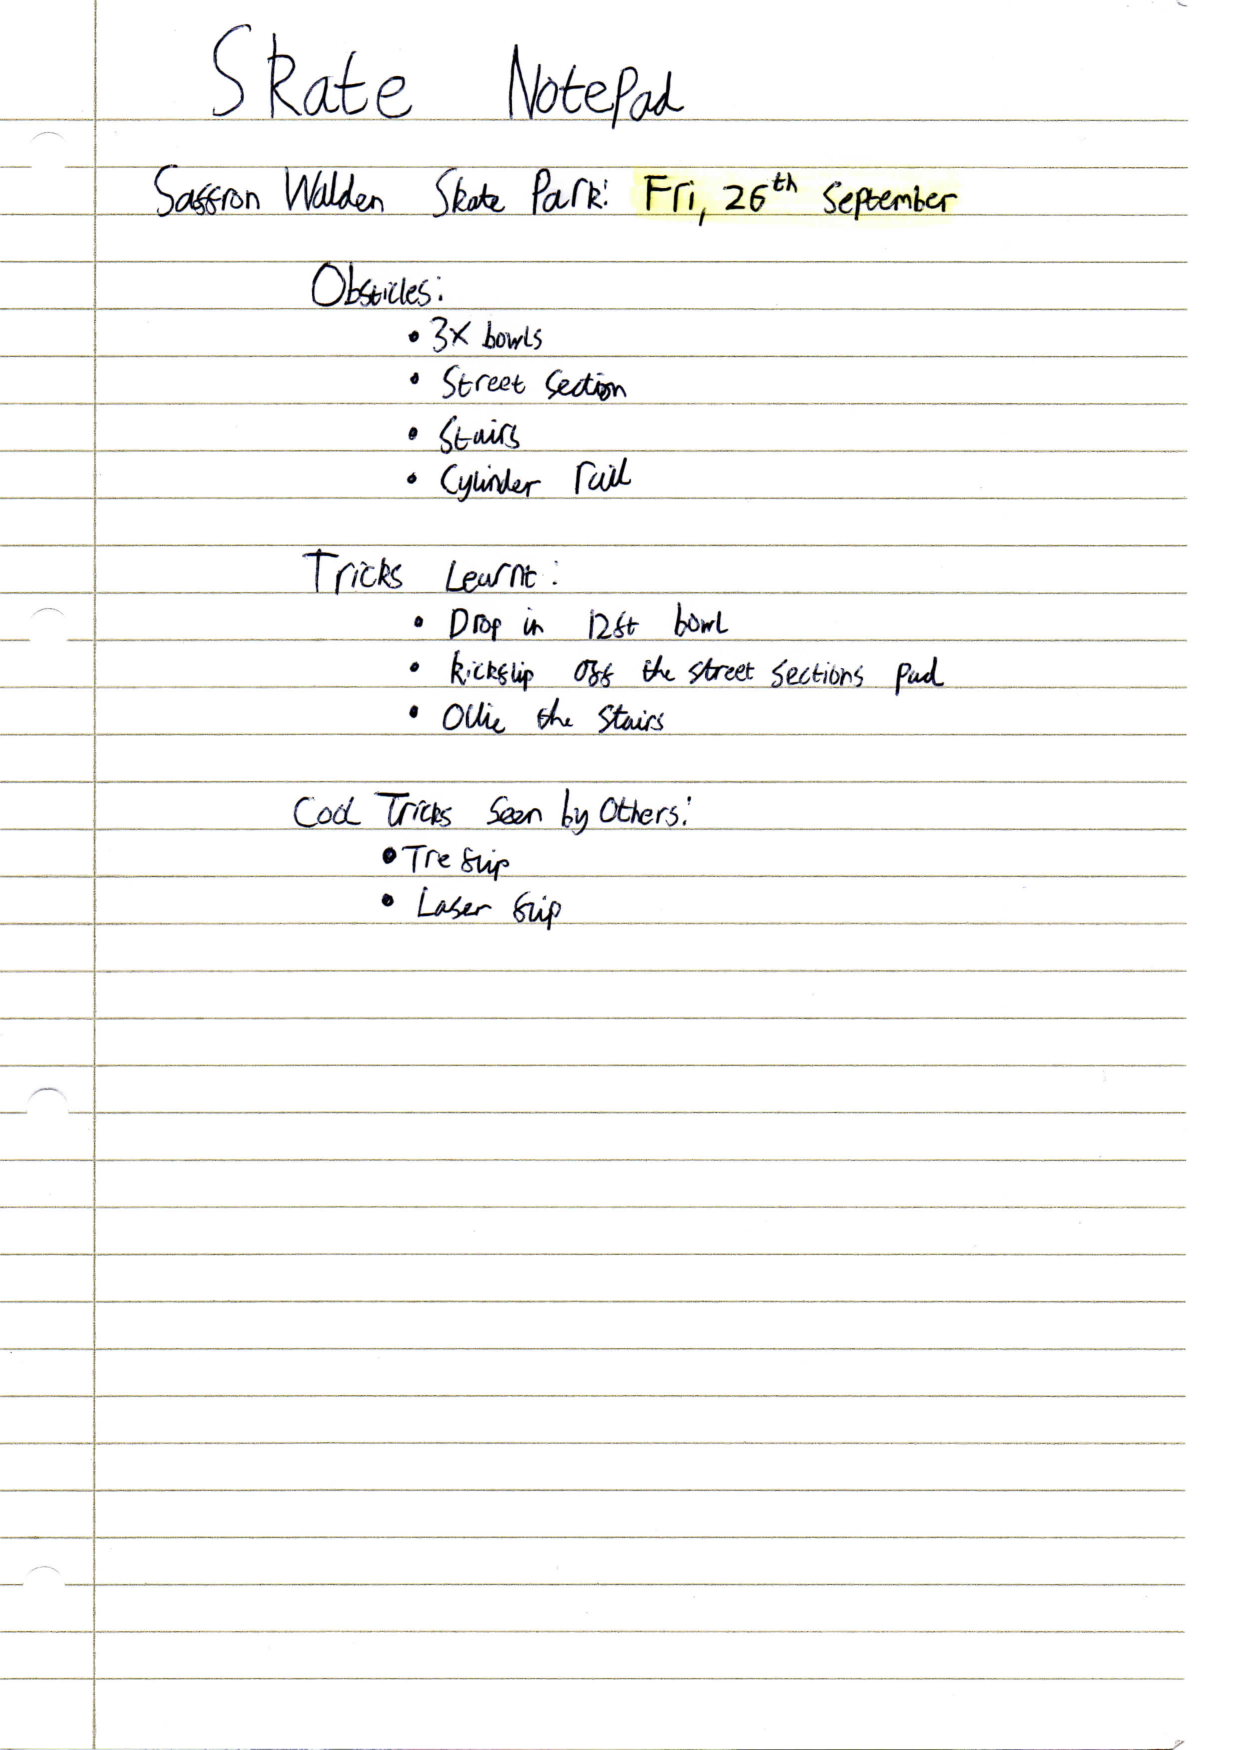
\includegraphics[width=\textwidth]{./Analysis/Notepad.pdf}
    \caption{A page from Stuarts notepad} \label{fig:Notepad Page}
\end{figure}

The only output forms in the current system would be the YouTube video links at redirect you to the YouTube video. A couple of these output links are listed below:

\begin{itemize}
\item How To Ollie Tutorial -  \url{https://www.youtube.com/watch?v=FuyYBWuV7VU&index=1&list=PLIZKb9hZiA_uFdK_zu9d_E_8gydHx5kwy}
\item How To Kickflip Tutorial -  \url{https://www.youtube.com/watch?v=_7fEsZG1xuI&index=2&list=PLIZKb9hZiA_uFdK_zu9d_E_8gydHx5kwy}
\end{itemize}

\subsection{The proposed system}

\subsubsection{Data sources and destinations}

The new system keeps some of the same data sources and destinations as the current system. For example YouTube will still be the source of the tutorial videos and google maps will still be used as the basis for mapping. But all of the other data will be stored internally within the system to increase the ease of access. 
\begin{center}
\begin{tabular}{|p{3cm}|p{3cm}|p{3cm}|p{3cm}|}
    \hline
 \textbf{Data Source} & \textbf{Data} & \textbf{Data Example} & \textbf{Data Destination}\\ \hline
User & Searching for a skatepark name & Cambourne skatepark & Google Maps Servers \\ \hline
Google Maps Server & Image of the location, coordinates, description & Image of Cambourne skatepark, 52.2200 N, 0.0700 W, Cambourne skatepark was established in 2002 & user \\ \hline 

User & Trick & Kickflip & Trick Database \\ \hline
User & Trick Description & Board rotating 360 degrees on a horizontal axis & Trick Database  \\ \hline
User & Trick Image & Kickflip.jpeg & Trick Database \\ \hline
User & Trick Tutorial Link & \url{ http://www.youtube.com/watch?v=1082h} & Trick Database \\ \hline


Trick Database & Trick & Kickflip & User \\ \hline
Trick Database & Trick Description & Board rotating 360 degrees on a horizontal axis & User  \\ \hline
Trick Database & Trick Image & Kickflip.jpeg & User \\ \hline
Trick Database & Trick Tutorial Link & \url{http://www.youtube.com/watch?v=1082h} & User \\ \hline

User & ProductName &  Trucks & Review Database \\ \hline 
User & Product Type & Trucks & Review Database \\ \hline
User & Product Size & 5.0 & Review Database \\ \hline
User & Product Brand & Thunder & Review Database \\ \hline
User & Product Review & Best Trucks I've owned & Review Database \\ \hline 
User & Product Rating & 1 & Review Database \\ \hline 

Review Database & Product Name & Spec ops & User\\ \hline 
Review Database & Product Type & Trucks & User \\ \hline
Review Database & Product Size & 5.0 & User \\ \hline
Review Database & Product Brand & Thunder & User \\ \hline
Review Database & Product Review & Best Trucks I've owned & User \\ \hline 
Review Database & Product Rating & 1 & User \\ \hline 





\end{tabular}
\label{tab:Proposed System Data Source and Destinations}
\end{center}












\subsubsection{Data flow diagram}


\begin{figure}[H]
    \includegraphics[width=\textwidth]{./Analysis/NewReviewSearch.pdf}
    \caption{Data flow diagram for the new systems review search} \label{fig:Review search}
\end{figure}



\begin{figure}[H]
    \includegraphics[width=\textwidth]{./Analysis/AddingTricksToDatabase.pdf}
    \caption{Data flow diagram for adding new tricks to the database} \label{fig:Adding tricks to database}
\end{figure}



\begin{figure}[H]
    \includegraphics[width=\textwidth]{./Analysis/ReadingTricksFromDatabase.pdf}
    \caption{Data flow diagram for reading tricks from the database} \label{fig:Reading tricks from database}
\end{figure}



\begin{figure}[H]
    \includegraphics[width=\textwidth]{./Analysis/NewTutorialSearch.pdf}
    \caption{Data flow diagram for the new systems tutorial search} \label{fig:Tutorial search}
\end{figure}



\begin{figure}[H]
    \includegraphics[width=\textwidth]{./Analysis/SkateparkSearch.pdf}
    \caption{Data flow diagram for the new systems skate park search} \label{fig:Skate park search}
\end{figure}










\begin{landscape}

\subsubsection{Data dictionary}
\begin{center}
\begin{tabular}{|p{3cm}|p{2cm}|p{2.5cm}|p{2cm}|p{3cm}|p{3cm}|}
    \hline
 \textbf{Name} & \textbf{Data Type} & \textbf{Length} & \textbf{Validation} & \textbf{Example Data} & \textbf{Comment} \\ \hline

TrickName & String & 25 characters & None & Ollie & Linked to Description, image and tutorial link \\ \hline
TrickDescription  & String & 100 characters & None & Board is turned around 180 degrees & Linked to trick, image and tutorial link \\ \hline
TrickImage & Image & N/A & 670 x 503 & Ollie.jpeg & None \\ \hline
TrickTutorialLink  & String & 100 characters & Correct link & \url {http://www.youtube.com/watch?v=3809} & Linked to trick, description and image \\ \hline
TrickDifficulty & string & 6 characters & easy, medium, hard & easy & colour coded \\ \hline
TrickCompleted & Boolean & True/False & None & True & None \\ \hline

SkateparkName & String & 25 characters & Correct Name & Cambourne Skatepark & None  \\ \hline
SkateparkCoordinates  & Float & 20 characters & Correct coordinates & 52.2200 N, 0.0700 W & None  \\ \hline
SkateparkDescription & String & 200 characters & Accurate description & Halfpipe only & None \\ \hline

ProductBrand & String & 20 characters & None & ZERO & Moderated \\ \hline
ProductType & String & 20 characters & None & Deck & Moderated \\ \hline
ProductName & String & 25 characters & None & Cosmic Tiger & Moderated \\ \hline
ProductSize & String & 20 characters & None & 7.875" & Moderated \\ \hline
ProductReview  & String & 500 characters & Non-biased & These trucks are the best I have owned & Moderated \\ \hline
ProductRating & interger & range 1-5 & Non-biased & 1 & Moderated \\  \hline


\end{tabular}
\label{tab:Proposed System Data Source and Destinations}
\end{center}
\end{landscape}


\subsubsection{Volumetrics}

For the initial size of the propsed system I chose to add 50 standard skate boarding tricks as there are limitless tricks and the user is able to add tricks to his own individual database of tricks and my client requested it (See the section appendix question 24). The maximum length of a name for a skateboarding trick is 25 characters, this is because they range from words such as "shuv" to "triple doliphin late flip". With the initial program as there will be 30 standard skateboarding tricks the names of them alone would take up 750 bytes as a string takes up 1 byte per character. The tickbox next to the trick stating whether you have completed the trick or not would take a boolean value and therefore take up 60 bytes of storage as boolean values take up 2 bytes each. The description of a trick would approximately be 100 characters, for example the description of a kickflip would be:

\begin{itemize}
\item  Flipping the board 360 $^{\circ}$  along the axis that extends from the nose to the tail of the deck.
\end{itemize}

This will add a further 3000 bytes to the program. The location coordinates of the skatepark will have to be stored, and the skateparks and spots around Cambridge is roughly 20 and each skatepark will contain 2 integers (the coordinates) and as integers take up 4 bytes of storage each the stored coordinates will initially be 160 bytes. The maximum length of YouTube link would be 100 characters and as there are 50 tricks already implemented there will be 50 links, this ultimately adds up to a further 5000 bytes.
images will be 670x503 which totals to 337010 bytes each and a total of 50 images will be needed which means in total 16850500 bytes if memory will be needed for images. 


Adding up all of the bytes of data would be calculated by the sum:

750+60+3000+160+5000+16850500 = 16859470Bytes 

To get this unit in KB you would divide the number of bytes by 1024 which equals 16464.3 KB (Rounded to 1 d.p)

To get this unit in MB you would divide by a further 1024 which equals 16.1 MB (Rounded to 1 d.p)

As this system will be ever expanding in the number of tricks that are added to the database the actual systems data size will be larger as time goes on.

\section{Objectives}

\subsection{General Objectives}

\begin{itemize}
\item Aesthetically pleasing, easy to navigate GUI.
\item Videos organised and filtering capabilities.
\item Correct and accurate mapping to the skate parks/spots.
\item Correct directions from current location to skate park/ spot on the map.
\item Non-biased reviews.
\item Clear database with a list of tricks in.
\item Easy to filter through tricks known.
\end{itemize}

\subsection{Specific Objectives}


\begin{itemize}
\item Ensure that videos can be filtered by categories. e.g easy, medium, hard tricks.
\item Ensure that videos load correctly and are linked to the right video.
\item Ensure that videos are displayed at the correct size/resolution that the monitor of the computer is.



\item Ensure the database can add, edit and remove trick data (Name, description, image, completed status and tutorial link).
\item Ensure that the database is displayed correctly inside the application at all resolutions.
\item Ensure that the tricks are marked by how hard they are by a three way scale of: Easy, Medium or Hard.
\item Ensure a checkbox is by the side of a trick to represent whether the user has completed that trick or not.
\item Ensure there is a search bar for a specific trick name.
\item Ensure there are filters for tricks e.g Switch trick filters.



\item Ensure that the map is accurate to current roads.
\item Ensure location of the user is not revealed to anyone else.
\item Ensure that the current location marker is accurate.
\item Ensure that when giving directions to skate parks from your current location that the mapping route is correct and on viable roads. 
\item Ensure that the program can mark skate park locations.




\item Ensure no biased reviews are posted to the app and that they're moderated before they are universally posted.
\item Ensure the program runs fast without lag when navigating between areas of the application.
\end{itemize}

\subsection{Core Objectives}

\begin{itemize}
\item Ensure that videos can be filtered by categories. e.g easy, medium, hard tricks.
\item Ensure that videos load correctly and are linked to the right video.
\item Ensure the database can add, edit and remove trick data (Name, description, image, completed status and tutorial link).
\item Ensure that the tricks are marked by how hard they are by a three way scale of: Easy, Medium or Hard.
\item Ensure a checkbox is by the side of a trick to represent whether the user has completed that trick or not.
\item Ensure there is a search bar for a specific trick name.
\item Ensure there are filters for tricks e.g Switch trick filters.
\item Ensure that the program can mark skate park locations.
\item Ensure the program runs fast without lag when navigating between areas of the application.
\end{itemize}

\subsection{Other Objectives}

\begin{itemize}
\item Ensure that videos are displayed at the correct size/resolution that the monitor of the computer is.
\item Ensure that the database is displayed correctly inside the application at all resolutions.
\item Ensure that the map is accurate to current roads.
\item Ensure location of the user is not revealed to anyone else.
\item Ensure that the current location marker is accurate.
\item Ensure that when giving directions to skate parks from yout current location that the mapping route is correct and on viable roads. 
\item Ensure no biased reviews are posted to the app and that they're moderated before they are universally posted.
\end{itemize}

\section{ER Diagrams and Descriptions}

\subsection{ER Diagram}


\begin{figure}[H]
    \includegraphics[width=\textwidth]{./Analysis/EntityRelationships.pdf}
    \caption{Entity-Relationship Diagram} \label{fig:Entity Diagram}
\end{figure}


\subsection{Entity Descriptions}

User({\underline{UserID}, Username}) \\ \\
Trick({\underline{TrickName},\emph{UserID},\emph{ Description}, \emph{Difficulty}, \emph{Completed},\emph{ Image}, \emph{TutorialLink}) \\ \\
Skatepark({\underline{SkateparkID},\emph{UserID}, \emph{ SkateParkName}, \emph{Coordinates}, \emph{Description}) \\ \\
Review({\underline{ReviewID}, \emph{UserID}, \emph{ReviewRating},\emph{ ProductName},\emph{ ProductType},\emph{ ProductSize}, \emph{ ProductBrand},\emph{Review}) \\ \\

UserTrick(\underline{UserTrickID}, \emph{UserID}, \emph{ Description},\emph{ Difficulty}, \emph{Completed},\emph{ Image}, \emph{TutorialLink}) \\ \\

UserSkatepark(\underline{UserSkateparkID}, \emph{UserID},   SkateParkName, Coordinates, Description) \\ \\

UserReview(\underline{UserReviewID}, \emph{UserID},  ReviewRating, ProductName, ProductType, ProductSize,  ProductBrand, Review) \\



\section{Object Analysis}

\subsection{Object Listing}

\begin{itemize}
\item User
\item Trick
\item SkatePark
\item Review
\item Product 

\end{itemize}

\subsection{Relationship diagrams}

\begin{figure}[H]
    \includegraphics[width=\textwidth]{./Analysis/RelationshipDiagram.pdf}
    \caption{Relationship Diagram} \label{fig:Relationship Diagram}
\end{figure}

\subsection{Class definitions}

\begin{center}
\begin{tabular}{|p{5cm}|}
    \hline
 \textbf{User} \\ \hline
UserID\\
Username \\ \hline
get\_user\_id \\
get\_username \\
\\ \hline 
\end{tabular}
\label{tab:User Class Definition}
\end{center}

\begin{center}
\begin{tabular}{|p{5cm}|}
    \hline
 \textbf{Trick} \\ \hline
TrickName\\
TrickDescription \\
TrickDifficulty \\
TrickCompleted \\
TrickImage \\
TrickTutorialLink \\ \hline

get\_trick\_name \\
get\_trick\_difficulty \\
get\_trick\_state \\
get\_trick\_image \\
get\_trick\_tutorial\_link
\\ \hline 
\end{tabular}
\label{tab:Trick Class Definition}
\end{center}

\begin{center}
\begin{tabular}{|p{5cm}|}
    \hline
 \textbf{SkatePark} \\ \hline
SkateParkID \\
SkateParkName \\
SkateparkCoordinates\\
SkateparkDescription 
\\ \hline 

get\_skatepark\_id
get\_skatepark\_name
get\_skatepark\_coordinates
get\_skatepark\_description
\\ \hline

\end{tabular}
\label{tab:Skate Park Class Definition}
\end{center}

\begin{center}
\begin{tabular}{|p{5cm}|}
    \hline
 \textbf{Review} \\ \hline
ReviewID\\

\\ \hline 

get\_review\_id \\

\hline

\end{tabular}
\label{tab:Review Class Definition}
\end{center}

\begin{center}
\begin{tabular}{|p{5cm}|}
    \hline
 \textbf{Product} \\ \hline
ProductName \\
ProductSize\\
ProductBrand \\
ProductType \\
ProductReview \\
\\ \hline 

get\_product\_name \\
get\_product\_size \\
get\_product\_brand \\
get\_product\_type \\
get\_product\_review \\
\hline

\end{tabular}
\label{tab:Review Class Definition}
\end{center}




\section{Other Abstractions and Graphs}


\begin{figure}[H]
    \includegraphics[width=\textwidth]{./Analysis/SkateparkMapping.pdf}
    \caption{Graph to show how the user can map their current location to skateparks.} \label{fig:Skatepark Graph}
\end{figure}














\section{Constraints}

\subsection{Hardware}

The new system will need to be able to run on Stuart's computer, the current specifcation of Stuart's laptop is:
\begin{itemize}
    \item 15.6" HD 1366x768 Screen
    \item i5-2450M Dual Core Processor (Sandy Bridge) 2.5GHz (overclocked to 3.1GHz) 3MB Cache
    \item 8GB DDR3 RAM
    \item 500GB HDD Memory
    \item Intel HD3000 Graphics Card
\end{itemize}

Stuarts laptop has more than enough processing power in order to run the new system, this will allow Stuart to run several applications whilst also using the new system. Stuart will be able to take the application with him wherever he takes his laptop. Therefore portability of the application isn't limited as he works on a laptop.

The only constraints will be the screen resolution and battery of his laptop, therefore optimising the program for his specific resolution will be a task to overcome and making the program universal for other users to run the program.

\subsection{Software}

Stuarts laptop is currently running on Windows 7 Home Premium, he does not want to have to install a virtual machine to run the application; however he does not mind installing external software to aid the systems running capability and ease. The new system however was initially thought to run on Windows 7 Home Premium and therefore this is not an issue. Stuart being willing to install extra programs gives some extra flexibility with how to overcome other problems if they arise. Therefore currently there are no foreseeable constraints regarding software.

\subsection{Time}

Currently the only time restriction is the project deadline, this is Friday 13h February 2015 for the implementation section of the coursework, this was set by my teacher. Stuart is extremely flexible with time and isn't under any time constraints as long as the final product works. 

\subsection{User Knowledge}

As an ex-computing student and a person regularly around computers, Stuart's knowledge about computers and the way that they work is good and therefore he is capable of understanding and explaining complex processes. This means that in the designing process of the new system I will be able to plan for keyboard shortcuts and more complex features which will essentially .  

\subsection{Access restrictions}

Restricting the data about the individual's location is an important feature of the application, other than that the information that is inputted into the system is general and therefore it does not need its access restricted. This lack of access restriction is in place as other users should be able to benefit from the skate parks and spots that another user has found. Due to the system not containing private information about a living individual, the new system will have no problems with any current legislation or law. 

\section{Limitations}

\subsection{Areas which will not be included in computerisation}

The process of learning tricks will still have to be done physically as it cannot be completed any other way, the same goes for seeing other people's tricks and being inspired to learn a new trick. Apart from that, all of the information will be stored in the system electronically and processed by the computer. 

\subsection{Areas considered for future computerisation}
\begin{itemize}
\item A forum for users of the app to discuss problems, help each other and recomend products.
\item Phone app.

\end{itemize}

\section{Solutions}

\subsection{Alternative solutions}


\begin{center}
\begin{longtable}{|p{5cm}|p{5cm}|p{5cm}|}
    \hline
 \textbf{Solution} & \textbf{Advantages} & \textbf{Disadvantages} \\ \hline
Web-Based Application 

& 
\begin{itemize}
\item Can access anywhere with an internet connection/LAN connection.
\item No installation required.
\item Nice formatting and extremely versatile.
\item Can use a lot of different programming languages to accomplish a task (HTML, CSS, JavaScript, PHP etc.)
\end{itemize}
 &
\begin{itemize}
\item  Lack of experience in web based programming.
\item More complex security for hiding locations.
\item Web Hosting costs money.
\item More extensive knowledge to fix problems.
\end{itemize}
\\ \hline
\begin{itemize}
\item Making the current system more efficient
\end{itemize}

& 
\begin{itemize}
\item No need for the client to learn anything new.
\item No expense.
\end{itemize}

&
\begin{itemize}
\item  Problems with the current system will still exist.
\item The system won't be as efficient.
\end{itemize}
\\ \hline

Command-Line Application

& 
\begin{itemize}
\item Runs extremely fast.
\item Uses minimal system resources.
\end{itemize}

& 
\begin{itemize}
\item Client will need to learn code.
\item Security would be hard to keep as there are 'hidden' codes.
\item No GUI.
\item Coding error could break the computer. 
\end{itemize}
\\ \hline

SQL Database

& 
\begin{itemize}
\item Runs complex queries fast.
\item Could store all the information in a compressed form.
\item Information easy to access.
\end{itemize}

& 
\begin{itemize}
\item No GUI.
\item Client would have to learn SQL code.
\item I am not very good at SQL code.
\item Debugging would be difficult.
\end{itemize} \\ \hline

Python Application with GUI (PyQt4)

& 
\begin{itemize}
\item Python is my primary programming language. 
\item Easy to use for the client.
\item Nice, clean GUI.
\item Versatile GUI and Python allows for the program to work on all types of systems.
\item Easy to format data.
\end{itemize}

& 
\begin{itemize}
\item Uses system resources more than other solutions.
\item Programming can be complex (GUI is harder than command-line). 
\end{itemize}
\\ \hline



\end{longtable}
\label{tab:Solutions to the problem}
\end{center}



\subsection{Justification of chosen solution}

I have chosen to complete the new system using a Python application with a PyQt Graphical User Interface.  I have chosen to create the system in this way as python is a programming language that is extremely versatile and will be able to carry out all of the tasks whilst supplying the client with a smooth and efficient experience. A web-based solution would not be appropriate as neither the client nor I am willing to pay to set up a server and also I do not have extensive knowledge and experience with working with programming languages such as: HTML, CSS, JavaScript and PHP. Making the current system more suitable would not be suitable either as the main problems with the current system would still appear in the new system, the client and I do not see this to be a worthy way to tackle this system. A command-line application would be too complicated for everyday use due to its steep learning curve and additionally the security threats are too high. Finally an SQL database doesn't provide a clean GUI like the python solution does and isn't as versatile in the ways that you can input and read data, which leaves me to believe that using the Python application is the most suitable for undertaking the new system. Python also contains extensive forums with information to help the client add any additional features he wants when my project is completed whilst also aiding me to find the best way to tackle the problems that I will encounter when programming the new system.


